\documentclass[11pt,a4paper]{article}

\usepackage[margin=2.4cm]{geometry}
\usepackage[T1]{fontenc}
\usepackage[utf8]{inputenc}
\usepackage{lmodern}
\usepackage{setspace}
\usepackage{booktabs}
\usepackage{graphicx}
\usepackage{float}
\usepackage{hyperref}
\usepackage{enumitem}
\usepackage{xcolor}

\hypersetup{
    colorlinks=true,
    linkcolor=black,
    urlcolor=blue,
    citecolor=black,
    pdftitle={Climate Suitability Analysis for Outdoor Wellness Tourism in Portugal},
    pdfauthor={Alice Mota}
}

\graphicspath{{figures/}}
\onehalfspacing
\setlength{\parindent}{0pt}
\setlength{\parskip}{0.65em}

\title{\textbf{Climate Suitability Analysis for Outdoor Wellness Tourism in Portugal}\\
\large Weather-Based Site Selection for a Mountain Wellness Retreat}
\author{Alice Mota}
\date{July 2026}

\begin{document}

\maketitle

\begin{abstract}
This report compares Guarda and Vila Real as candidate locations for a mountain wellness retreat in Portugal. The analysis uses daily meteorological data from 2018-01-01 to 2026-02-28 and evaluates each city using a business-oriented definition of a weather-suitable retreat day. The results support Guarda as the stronger location for outdoor wellness tourism because it provides more suitable days per year, fewer rain days, and fewer hot days than Vila Real. Vila Real remains attractive for milder winter conditions, but its higher rain and heat exposure makes it less reliable for outdoor retreat programming.
\end{abstract}

\section{Business Question}

The client needs to choose between two inland mountain cities in Portugal: Guarda and Vila Real. The central business question is:

\begin{quote}
\textbf{Which city offers the stronger weather profile for an outdoor mountain wellness retreat, and during which months should the business prioritize outdoor programming?}
\end{quote}

This is a site-selection problem rather than a purely meteorological comparison. A suitable location must support guest comfort, reliable outdoor activities, seasonal programming, and manageable weather-related operating risk.

\section{Dataset Description}

The analysis uses two daily weather datasets:

\begin{itemize}[leftmargin=*]
    \item \texttt{dataset/raw\_GUARDA.csv}
    \item \texttt{dataset/raw\_VILA\_REAL.csv}
\end{itemize}

Together, the files contain 5,962 daily observations, evenly split between the two cities. The date range is 2018-01-01 to 2026-02-28. The main variables include maximum, minimum, and mean temperature; precipitation; wind speed; wind gusts; sunshine duration; shortwave radiation; relative humidity; cloud cover; latitude; and longitude.

The 2026 observations are partial and are therefore used in the processed daily dataset, but excluded from annual averages and model validation.

\section{Data Cleaning}

The cleaning process was implemented in \texttt{src/build\_analysis.py}. The pipeline:

\begin{itemize}[leftmargin=*]
    \item loads both city files and combines them into one daily dataset;
    \item standardizes city labels and column names;
    \item parses dates into datetime format;
    \item removes duplicate city-date records;
    \item validates that required weather fields contain no missing values;
    \item sorts observations by date and city.
\end{itemize}

No missing values were found in the required fields, which makes the comparison consistent across both cities.

\section{Feature Engineering}

The project creates several decision-oriented features:

\begin{itemize}[leftmargin=*]
    \item calendar features: year, month, month name, day of year, and season;
    \item sunshine hours, converted from raw sunshine duration;
    \item daily temperature range;
    \item rain day flag, based on precipitation of at least 1 mm;
    \item hot day flag, based on maximum temperature above 30$^\circ$C;
    \item freezing day flag, based on minimum temperature below 0$^\circ$C;
    \item windy day flag, based on wind gusts of at least 40 km/h;
    \item cyclic month and day-of-year features for modelling;
    \item binary target variable: \texttt{suitable\_retreat\_day}.
\end{itemize}

A day is classified as suitable for outdoor retreat programming when all of the following conditions are true:

\begin{itemize}[leftmargin=*]
    \item maximum temperature is between 18$^\circ$C and 30$^\circ$C;
    \item precipitation is below 1 mm;
    \item wind gusts are below 40 km/h;
    \item sunshine duration is at least 3 hours;
    \item average cloud cover is at or below 80\%.
\end{itemize}

These thresholds are intentionally simple and transparent. They can be adjusted if the business later defines a different comfort standard.

\section{Exploratory Analysis}

The descriptive results show that both cities can support outdoor wellness tourism, but their risk profiles differ.

\begin{table}[H]
\centering
\caption{Weather suitability scorecard, complete years 2018-2025}
\begin{tabular}{lrrrrrr}
\toprule
City & Suitable days & Suitability & Rain days & Hot days & Freezing days & Windy days \\
 & per year & rate & per year & per year & per year & per year \\
\midrule
Guarda & 74.4 & 20.4\% & 102.8 & 19.9 & 38.6 & 150.6 \\
Vila Real & 69.9 & 19.1\% & 124.8 & 33.8 & 8.0 & 153.2 \\
\bottomrule
\end{tabular}
\end{table}

Guarda has the stronger annual profile for outdoor retreat suitability. It records more suitable days per year, fewer rain days, and fewer hot days. Vila Real has fewer freezing days, which is an advantage for winter comfort, but this does not offset its higher rain and heat risk for an outdoor wellness concept.

\begin{figure}[H]
    \centering
    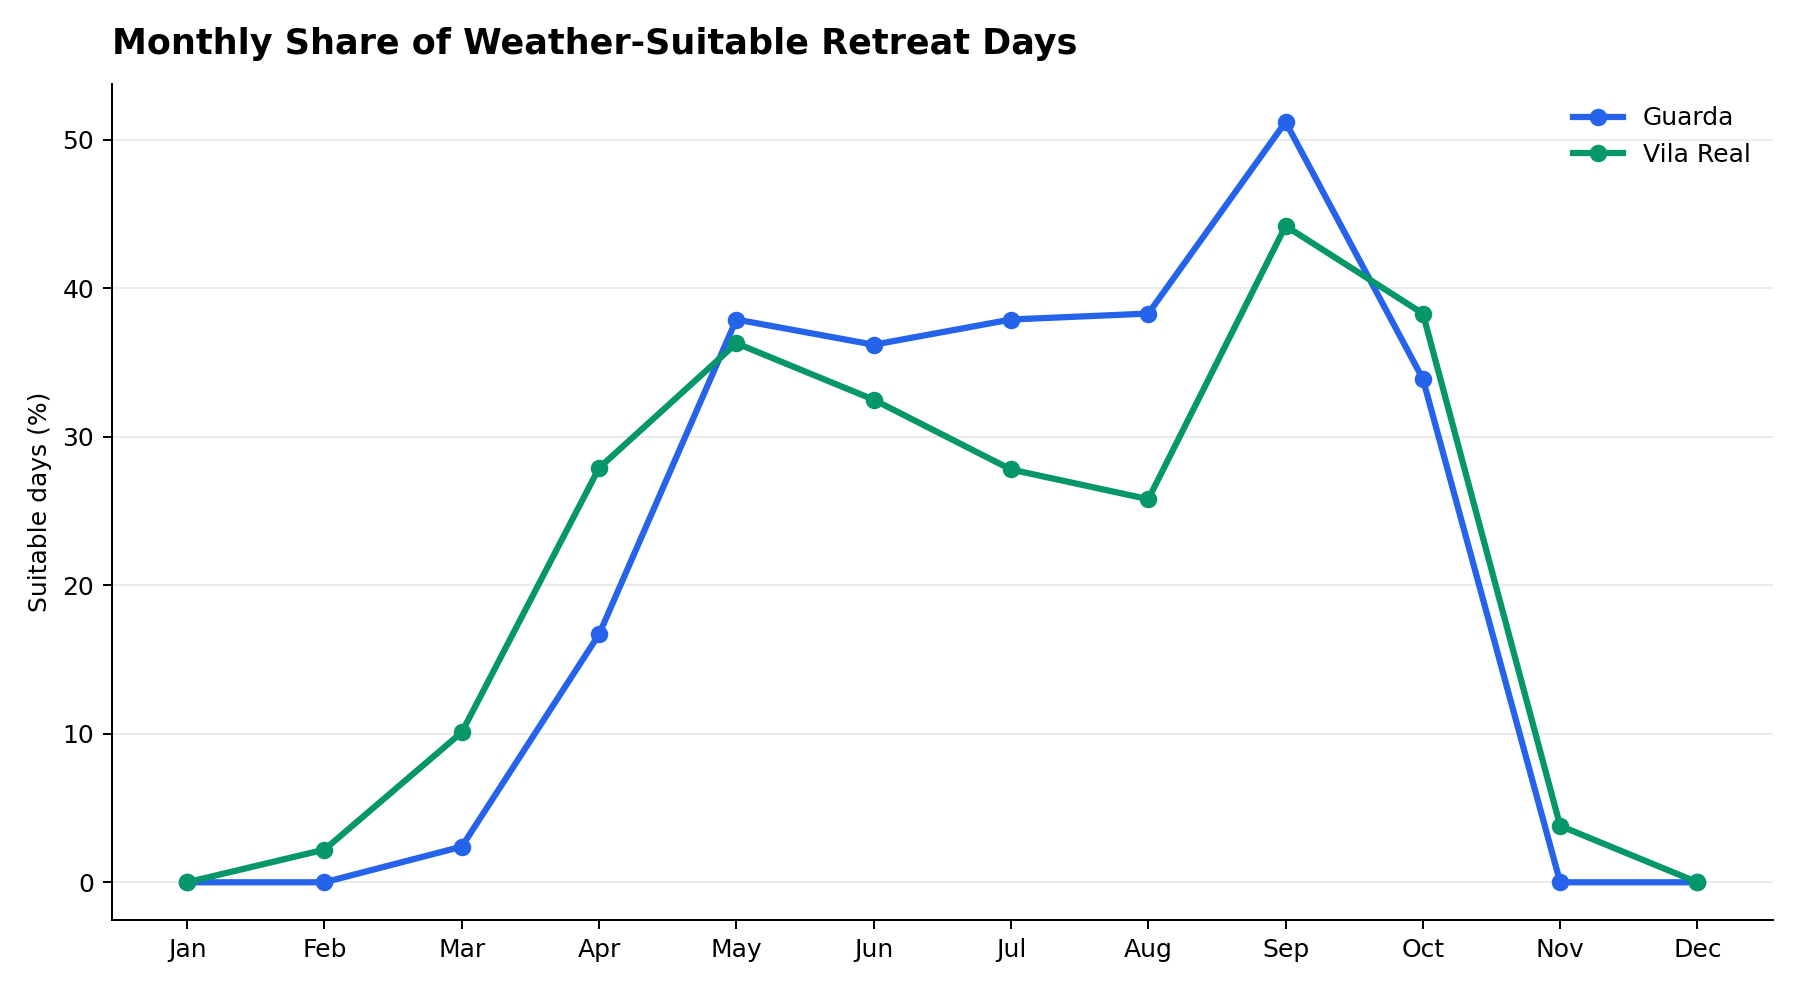
\includegraphics[width=0.92\textwidth]{monthly_suitability_rate.png}
    \caption{Monthly share of weather-suitable retreat days by city}
\end{figure}

\begin{figure}[H]
    \centering
    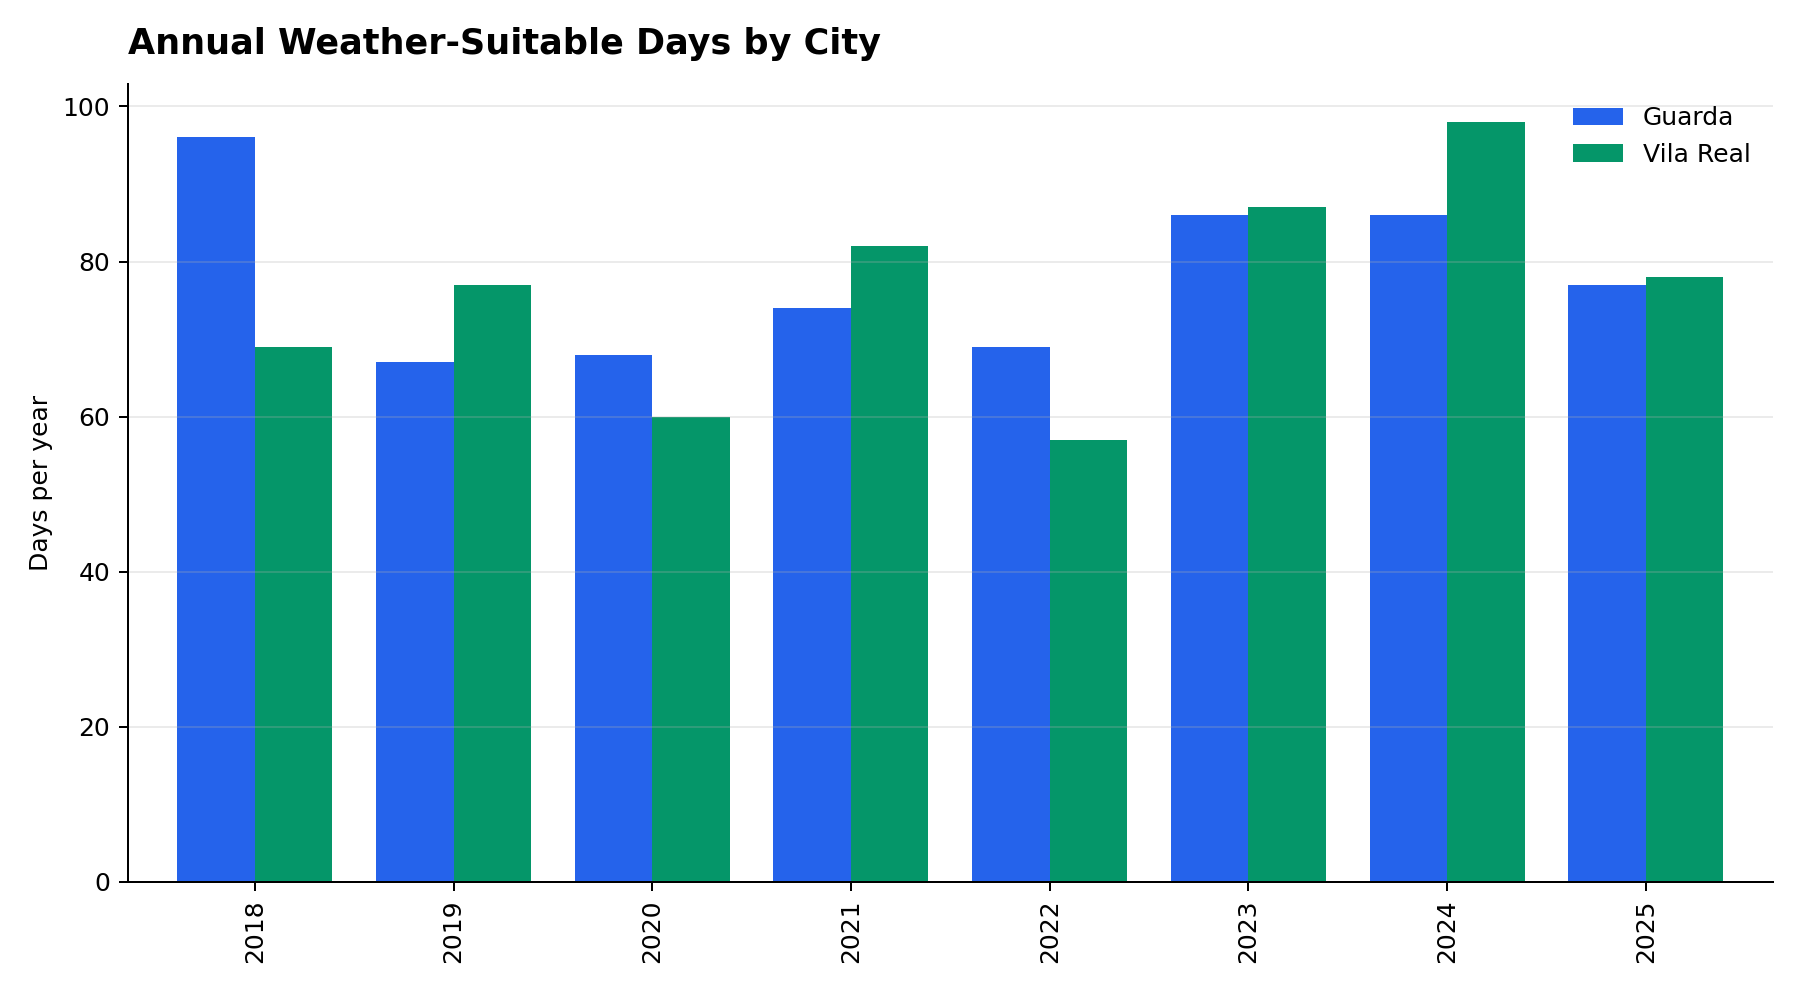
\includegraphics[width=0.92\textwidth]{annual_suitable_days.png}
    \caption{Annual count of weather-suitable retreat days by city}
\end{figure}

\section{Model Validation}

The modelling component is used to validate whether city and seasonal patterns contain useful planning signal. It is not designed as a real-time weather forecasting model.

Two classification models were trained using data from 2018-2024 and tested on 2025:

\begin{itemize}[leftmargin=*]
    \item Logistic Regression;
    \item Random Forest.
\end{itemize}

The models use planning features such as city, season, month, and cyclic date variables. They do not use same-day weather variables such as precipitation or temperature because those would make the prediction less useful for advance planning.

\begin{table}[H]
\centering
\caption{Model validation results on 2025}
\begin{tabular}{lrrrrr}
\toprule
Model & Accuracy & Precision & Recall & F1 & ROC AUC \\
\midrule
Logistic Regression & 0.674 & 0.366 & 0.896 & 0.520 & 0.778 \\
Random Forest & 0.655 & 0.350 & 0.875 & 0.500 & 0.816 \\
\bottomrule
\end{tabular}
\end{table}

The ROC AUC scores indicate that the seasonal and city-level variables contain meaningful signal. Precision is modest, which is expected because suitable days are relatively constrained and the model intentionally avoids using direct weather observations. For business use, the model is best interpreted as a planning support tool rather than a booking-day forecast.

\begin{figure}[H]
    \centering
    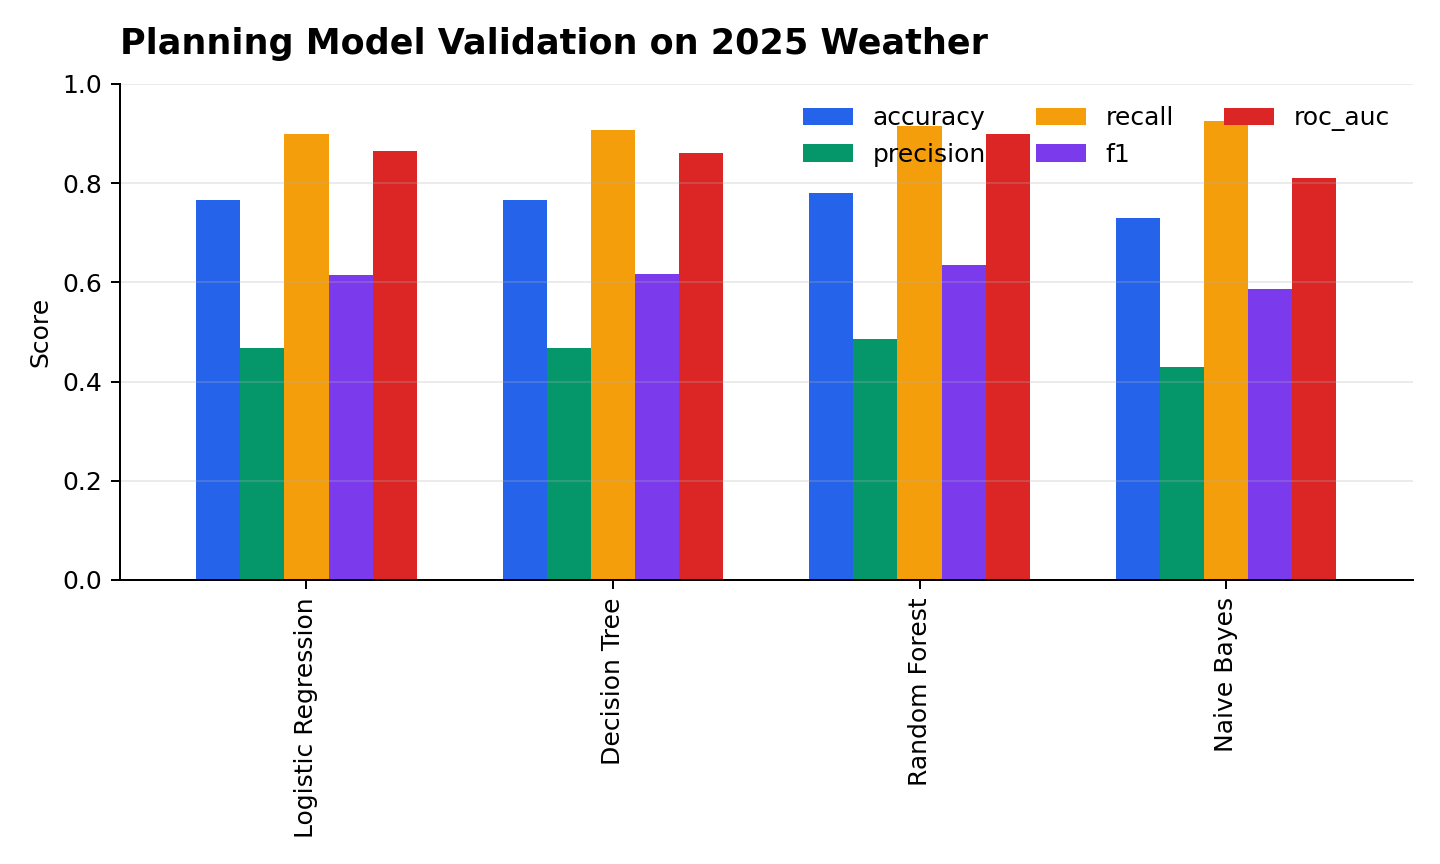
\includegraphics[width=0.82\textwidth]{model_validation.png}
    \caption{Validation performance for planning models}
\end{figure}

\section{Recommendation}

\textbf{Recommendation: choose Guarda as the preferred site for the mountain wellness retreat.}

Guarda is the stronger option for the proposed outdoor wellness concept because it offers:

\begin{itemize}[leftmargin=*]
    \item more weather-suitable retreat days per year;
    \item fewer rain days, reducing disruption to outdoor activities;
    \item fewer hot days, improving comfort for hiking, yoga, and nature-based activities;
    \item a clearer operational story for positioning the retreat around mountain climate and outdoor wellness.
\end{itemize}

Vila Real should not be dismissed entirely. It has fewer freezing days and may be more comfortable in parts of winter. However, the business model depends most strongly on reliable outdoor programming and comfortable activity conditions. Under that objective, Guarda has the stronger overall weather profile.

\section{Limitations}

The analysis has several limitations:

\begin{itemize}[leftmargin=*]
    \item only two candidate cities are compared;
    \item suitability thresholds are business assumptions and should be reviewed with stakeholders;
    \item the model validates seasonal planning patterns, not real-time weather forecasts;
    \item land cost, accessibility, accommodation supply, local partnerships, competition, and customer demand are not included;
    \item climate change scenarios are not modelled;
    \item 2026 data is partial and excluded from complete-year comparisons.
\end{itemize}

\section{Next Steps}

Before making an investment decision, the weather findings should be combined with:

\begin{itemize}[leftmargin=*]
    \item property and operating cost analysis;
    \item transport access from airports and major cities;
    \item tourism demand and competitor benchmarking;
    \item local supplier and activity partnership mapping;
    \item guest willingness-to-pay research;
    \item scenario testing with alternative weather suitability thresholds.
\end{itemize}

The current analysis provides a clear climate-based recommendation, but a final investment decision should combine weather suitability with commercial feasibility.

\end{document}
